\documentclass{emulateapj}

\usepackage{fullpage}
\usepackage{graphicx}

\shorttitle{Search for Extended LAT Sources}

\usepackage{amsmath}

\begin{document}

\title{Search for Spatially Extended Fermi-LAT Sources Using Two Years of Flight
Data}

\author{
J.~Lande\altaffilmark{3}, 
\altaffiltext{3}{W. W. Hansen Experimental Physics Laboratory, Kavli Institute for Particle Astrophysics and Cosmology, Department of Physics and SLAC National Accelerator Laboratory, Stanford University, Stanford, CA 94305, USA}
}


\begin{abstract}
We present a new method for analyzing spatially extended sources with
the Fermi Large Area Telescope (LAT), the primary science instrument
on the {\em Fermi Gamma-ray Space Telescope (Fermi)}.  We provide a
series of Monte Carlo studies that were done to validate this tool.
We then apply this tool to test all sources in the 2FGL Two Year Catalog
for extension.\cite{2FGL} We then report on the discovery of XXX new
extended sources.
\end{abstract}

\section{Introduction}

% * Resolving spatially extended Fermi sources is important for 
%    * studying supernova remnants, 
%    * pulsar wind nebulae, 
%    * galaxies,  
%    * potentially dark matter or new physics.
% * We searched all 2FGL catalog sources
% * Systematic test for a certain kind of (~ small) regularly shaped extended 

The Large Area Telescope (LAT) is a pair conversion telescope on the
Fermi Gamma-Ray Space Telescope that has been surveying the gamma ray
sky since June 2008.  Fermi is particuarly well suited for surveying
the entire Gamma-ray sky since it has a broad energy coverage (20MeV
and 300GeV), a wide field of view (~2.4 sr) and large effective area
($\approx 8000 \text{cm}^2$ at > 1GeV).

The LAT has been essential in understanding a variety of astrophysical
sources including Active Galactic Nuclei, Pulsars, and Supernova Remnants.
Many of the astrophysical sources seen by the Fermi LAT, espeically
galactic Supernova Remnants and Pulsar Wind Nebulae, can be resolved at
other wavelengths and could potentially be resolved by the LAT.

Resolving spatially extended GeV sources is important for studying a
variety of science topics. The most important use of spatial morphology
is in source identification. Many of the sources found in GeV sources

Nevertheless, morphological studies of sources in the GeV energy range using
the Fermi LAT is challenging primarily because of the significantly energy
dependent PSF and because of systematic errors in the
galactic diffuse emission. The Fermi PSF varies from over $XXXXX^\circ$
at 100MeV to $XXXXX^\circ$ at 100GeV and so the higher energy photons are

studying supernova remnants, 
pulsar wind nebulae, 
 * galaxies,  
 * potentially dark matter or new physics.

The Large Area Telescope (LAT) on the Fermi Gamma-Ray Space Telescope
has been surveying the Gamma-ray sky since August 2008. The LAT has been
been essential in studying a variety of astrophysical sources including
Active Galactic Nuclie, Pulsars, Supernova Remnants. 
One of the important data productes 

Using 11 months of data, the LAT produced the best-resolved survey of the sky
in the 100 MeV to 100 GeV energy range\cite{2FGL Paper}. The


\section{Analysis Method}


%   * Difficulty of studying spatially extended sources
%   * Pointlike, great features
%   * modifying it to fit spatially extended sources.
%      * semi-analytic convolution formula
%   * importance of fitting position + extension + spectrum simultaneously to apply statistical significance
%   * Monte Carlo Validation
%

Performing morphological studies of sources in the GeV energy range using
the Fermi LAT is challenging primarily because of the significantly energy
dependent PSF and because of systematic errors in the
galactic diffuse emission. The Fermi PSF varies from over $XXXXX^\circ$
at 100MeV to $XXXXX^\circ$ at 100GeV and so the higher energy photons are
significantly more important for studying the shape of sources. One could
ideally look just at the highest energy photons, but the trade off is that
for typical sources many more source events are expected at low energy.
For this reason, it is especially important to use as much of the data
as possible.

The second primary difficult in studying spatially extended sources is
systematic uncertainties in the diffuse emission. Systematic errors are
notoriously difficult and will be discussed more later, but the important
point to make here is that one of the most important diagnostic tools for
studying systematic errors is being able to iterate the analysis while
varying different parameters such as what goes into the diffuse model.

A new analysis tool has been developed to address these unique
requirements for studying spatially extended sources with the Fermi
LAT. The overall approach for this analysis is to perform a maximum
likelihood analysis where the Poisson likelihood for observing the
measured counts is computed given an assumed sky model. The parameters
of the sky model are then fit by maximizing the log of the likelihood.
To study the extension of a source, one can assume a particular shape
for an extended source (e.g. a disk or Gaussian), and fit the spatial
parameters of that source.

In principle, the entire task can be done using the standard science
tools package {\em gtlike}\cite{Science-Tools-gtlike}. But {\em gtlike} is
only able to fit the spectral parameters of the source, so the extension
fitting would have to be done as an external loop. Typically, the run time
for a binned source analysis using {\em gtlike} is several hours so this loop
would be especially time consuming. In principle, parallel computing could
ease this burdon, but parallel fitting algorithms are rather untested
and complex. Furthermore, the machinery required to do something like
this would necessarily be rather complex. What has typically been done by
the Fermi team to study extended sources is to fix the assumed position
of the extended source, either by our knowledge of a source from other
wavelenghts, or by fitting it as a point source. Then, a profile of the
likelihood as a function of extension is developed using {\em gtlike}
and the maximum of this profile. This approach is not optimal because it
needs not be the case that the best fit position of a point source would
be the same as the best fit position of an extended source. Furthermore,
by not fully maximizing the likelihood, this method is not as significant to
extension, especially of faint sources. And finally, since this approach
is so computationally intensive, no large scale Monte Carlo effort has been
launched to validate the method.

Instead, an alternate approach was developed for performing
a morphological analysis. An alternate maximum likelihood fitting
package called {\em pointlike} has been developed by the Fermi
collaboration and we have expanded its functionality to fully support
analyzing spatially extended sources. {\em pointlike} is most thoroughly
described in Matthew Kerr's Ph.D Thesis\cite{Matthew_kerr_phd_thesis}
but the important aspects will be summarized below. What differentiates
{\em pointlike} most significantly from {\em gtlike} is its emphasis
on speed by introducing approximations into the calculation of the
likelihood function while at the same time trying to reduce any
numerical errors that may be introduced.  Like binned {\em gtlike},
{\em pointlike} bins the sky both in position and energy.  Unlike {\em
gtlike}, pointlike relies on the {\em healpix} representation of spatial
bins\cite{healpix_paper} and scales the size of each spatial bin to be
smaller than the PSF. This is convenient because it no
significant information is lost due to binning at all energies and it is
always a good approximation that the model predicted counts are uniform
across a spatial bin. Furthermore, {\em pointlike} uses a sparse matrix
representation of the spatial bins where only the bins with counts in them
are looped over. The only downside to this is that the integral of the
model predicted counts must be independently calculated.  Effectively,
{\em pointlike} efficiently interpolates from a totally binned analysis
at low energy (where the resolution is poor and there are many counts)
to an unbinned analysis at high energy (where the resolution is very
good but there are few counts). This approach provides a significant
savings in time while introducing only small numerical error.

We have modified {\em pointlike} to support fitting spatially extended
sources.  To do this, we introduced a new class of diffuse sources where
the spatial and spectral information completely decouple and where
the spatial shape is parameters by simple objects (Disks, Gaussian).
The code consistently convolves the extended source shape with the point
spread function (as a function of energy) and integrates the spectrum over energy
to computed model predicted counts.

Finally, {\em pointlike} allows the spatial parameters of an extended
source to be simulataneoulsy fit. {\em pointlike} uses the Minuit fitting
library to perform the maximum likelihood maximization of the position
and extension of an extended source\cite{Minuit reference}.  At each
step in the fit of the shape, the spectral parameters of the entire sky
model are reoptimized. To avoid projection effects, what is directly
fit is not the longitude and latitude of the source but instead
the displacement in a rotated reference frame. The covariance matrix is
then computed and inverted to estimate the statistical errors on the
position and extension.

{\em pointlike} optimizes the analysis of extended sources in two ways.
First, for extended sources which are radially symmetric, the convolution
of the source shape with our parameterization of the PSF can be performed
semi-analytically. Generally, at a given energy the observed 
photon distribution is
\begin{equation}
  \text{PDF}(\vec r) = \int  \text{PSF}(|\vec r - \vec r'|)I_\text{src}(\vec r') d A' 
\end{equation}
where $I_\text{src}$ is the extended soruce shape and the PSF is parameterized by
\begin{equation}
  \text{PSF}(\vec r) = 
  \frac{1}{2\pi\sigma^2}
  \left(1-\frac{1}{\gamma}\right)
  \left(1+\frac{u}{\gamma}\right)^{-\gamma}
\end{equation}
Here, $\sigma$ and $\gamma$ are parameterize the $PSF$.
If the extended source is radially symmetric, then
$I_\text{src} (\vec r') = I_\text{src} (r')$ and the angular part of the
integral can be done analytically, leaving a simpler one dimensional
integral:
\begin{multline}
  \text{PDF}(u)= \int_0^\infty dv
  I_\text{src}(v) 
  \left(\frac{\gamma-1}{\gamma}\right)
  \left( \frac{\gamma}{\gamma + u + v}\right)^\gamma \\
  \times ~_2F_1 \left(\gamma/2,\frac{1+\gamma}{2},1,\frac{4uv}{(\gamma+u+v)^2}\right)
\end{multline}
Not only is this convolution formula faster, but it has the advantage
that it more accurately reduces to the actual PSF shape as the source's
size decreases.  Decreasing the numerical difference between a small extended
source and the PSF is important when searching for smaller extended sources
and when determining the statistical significance of a detection.

There is one final approximation which speeds up the convolution.
Generally, the PSF is a function of the angle $\theta$ of the incident
event measured relative to the normal to the LAT. To avoid repeatedly
convolving the source shape with the PSF at a series of $\theta$ angles,
an effective PSF is fit to the weighted sum of the PSF times the exposure
at different $\theta$ angles.  Since the source convolution has to be
done at each fit iteration, these optimization were essential for making
this tool fast enough for the following analysis. Typically, the entire
process of fitting the extension and estimating the errors for a source
would run on the order of an hour.

To calculate the statistical significance of the extension of a source,
one can define a parameter $\text{TS}_\text{ext}$ as twice the increase
in log likelihood between fitting a source with a
spatially extended hypothesis and a point hypothesis. 
So $\text{TS}_\text{ext}=2\times(LL_\text{ext}-LL_\text{ps})$.

In going from fitting a point source to fitting a simple extended source such as
a disk, the source's width is the only degree of freedom added to the model. According to
Wilk's Theorem, the distribution of $\text{TS}_\text{ext}$ for no signal (when there is a true
point source) should follow a $\chi^2_1$ distribution with one degree of freedom\cite{Wilks_Theorem}.
Wilk's Theorem only holds when the likelihood is maximized simultaneoulsy
fitting all of the parameters of model. It is for this reason why {\em pointlike}
goes through such great effort to simultaneously fit the position, extension,
and spectral paramters of a source.

On the other hand, since the null hypothesis rests on the edge of
parameter space, when the extension is fixed to 0, Wilk's Theorem does
not formally hold\cite{Warnings about Wilk's Theorem Paper}.  One might
expect the actual distribution to be a half $\chi^2_1$ distribution with
one degree of freedom plus half of a delta function at 0:
\begin{equation}
  P(\text{TS})=\tfrac{1}{2}(\chi^2_1(\text{TS})+\delta(\text{TS})).
\end{equation}
The false detection probability can be estimated by integrating this function 
from an observed test statistic value to infinity. It is for this
particular distribution that the often quoted result holds that
$\sqrt{TS}$ is a measure of the number of $\sigma$ of the detection.

The half $\chi^2_1$ distribution was found by a monte carlo study
to hold for the special case of source finding of EGRET sources using the
maximum likelihood technique.  They were comparing the hypothesis of a
source to the hypothesis of just a background\cite{Mattox_et_All_Paper}.
Their argument for why this null hypothesis distribution was reasonable
was that half of the time, statistical underfluctuations would cause
there to be fewer fewer photons then expected where the sources is being
tested. Since the maximim likelihood machinery cannot fit negative
sources (which would lead to negative model predicted for which the
poisson likelihood is undefined), half of the tests would not have the
likelihood improved by adding a source to the model and $\text{TS}=0$.
It is for the case that the null distribution has 

It seems plausable that a similar situation could happen for when testing
a source for extension. Half of the time, statistical flucutations might
make the observed counts narrower thant the point spread function and
the likelhood would not improve by fitting the source with an extended
hypothesis. We tested this hypothesis below using a dedicated monte
carlo study.

One issue that we found when testing this analysis method is that
despite our best efforts, there was always a small discrepancy between
the likelihood value when fitting the source as a point source and when
fitting it as an extended source with a small extension.  This is to be
expected due to numerical innacuracies introduced by the convolution.
For most cases, this error is insignificant. It would not significanlty
bias any of the fit values or errors. But it would bias the distribution
of $\text{TS}_\text{ext}$ in the null hypothesis. To correct for this,
instead of computing the likelihood in the null hypothesis by fitting
a point source, a new source model was introduced which is an extended
source with its extension fixed to a very small value. $LL_\text{ps}$
is then calculated by refitting this source using the same extended
source fitting code. It was only after introducing this change that we
were able to get broad agreement between simulations and Wilk's theorem.

\section{Monte Carlo Validation}

We performed a dedicated monte carlo study to validate pointlike for
studying spatially extended sources and also to demonstrate that we can
use $\text{TS}_\text{ext}$ as a test of the statistical significance
of a source's extension.  The monte carlo study involved simulating point
sources of varying spectral models on top of a simulated background. The
simulated point source was then fit using pointlike as both an extended
source and a point source and $\text{TS}_\text{ext}$ was calculated.

Fermi LAT data was simulated using the publically avaliabable Science
Tools package {\em gtobssim}\cite{GTOBSSIM_CITATION}. The sources were
simulated with a powerlaw spectral model with 6 Were given 6 $>100\text{MeV}$
fluxes ranging from $3\times 10^{-9} ph/cm^2/s$ to $10^{-6} ph/cm^2/s$.
The sources were then simulated with spectral index ($\gamma$) values of
1.5, 2, 2.5, and 3.  These values were picked to probe a representative
range measurable values.  For particular spectral indices, only the
fluxes which would create a statistically significant source detection
($\text{TS}>25$) where selected, since we are only interested in
testing for extension sources with a significant extent. The sources were
simulated on top of an isotropic powerlaw background with a Sreekumar-like
spectrum ($>\text{100MeV}$ flux of 1.5e-5 and spectral index 2.1).\cite{Sreekumar
et al. ApJ 494 pag 523 1998}

The monte carlo simulation was perforormed over a one year time interval using
a default rocking profile and an assumed livetime fraction of 0.8.
The reconstruction was perfromed with events from an energy range of
1GeV to 100GeV using 4 energy bins per decade and using the Pass 7 Version 6
source IRFs to be consistent with the following analysis.

For most of the spectral models, over 10,000 statistically independent simulations were performed.
For fainter sources, some of the simulated sources, statistical flucatuations
caused the source to be not significant and they were excluded from the following analysis.
Table~\ref{ts_ext_num_sims} shows the parametesr used in the simualtion,
the number of simulations perfromed, and the average test statistic value.

\begin{table}
  \begin{centering}
\begin{tabular}{ | r | r | r | r | }
\hline
$\gamma$ & flux ($ph/cm^2/s$) & $N_\text{sims}$ & $<\text{TS}>$ \\
\hline
  1.5 &          $10^{-6}$ &           11405 &  90861 \\
      &  $3\times 10^{-7}$ &           11490 &  21922 \\
      &          $10^{-7}$ &           11101 &   5765 \\
      &  $3\times 10^{-8}$ &           10269 &   1262 \\
      &          $10^{-8}$ &            9941 &    306 \\
      &  $3\times 10^{-9}$ &           10427 &     61 \\
\hline
    2 &          $10^{-6}$ &           11632 &  22025 \\
      &  $3\times 10^{-7}$ &           11622 &   4886 \\
      &           $1^{-7}$ &           11115 &   1159 \\
      &  $3\times 10^{-8}$ &           10503 &    222 \\
      &           $1^{-8}$ &            9893 &     50 \\
\hline
  2.5 &          $10^{-6}$ &           11522 &   4722 \\
      &  $3\times 10^{-7}$ &           11445 &    948 \\
      &           $1^{-7}$ &           10966 &    202 \\
      &  $3\times 10^{-8}$ &            8227 &     41 \\
\hline                                                
    3 &          $10^{-6}$ &           11264 &    949 \\
      &  $3\times 10^{-7}$ &           10986 &    172 \\
      &           $1^{-7}$ &            7855 &     40 \\
\hline
\end{tabular}
\caption{List of the spectral models used to the monte carlo simulation of
{\em pointlike}.$N_\text{sims}$ is the number of monte carlo simluations
which produce a significant source detection.The final column is the
average test statistic that was found during the monte carlo fit of
the source. Only simluations which were deemed significant ($\text{TS}>25$)
were kept.}
\label{ts_ext_num_sims}
  \end{centering}
\end{table}

The results of the monte carlo simulation are shown in
figure~\ref{ts_ext}.  The cumulative density function (CDF) is plotted
against $\text{TS}_\text{ext}$ For reference, the CDF for $\chi^2_1/2$,
suggested by Wilk's Theorem, is also plotted for comparison. Overall,
there is good agreement between Wilk's theorem, although the agreement
is not perfect.  Possible reasons for departure from Wilk's theorem may
include pointlike ignoring energy dispersion, which would generally change
the shape as a function of energy, numerical innacuracies in evaluating
the convolution algorithm, or possibly problems with the fitting algorithm
getting stuck in false minimum. It is important to emphasize that if
our emperical curve lies to the left of the curve we assume to estimate
significance, we would underestimate the statistical significance of
our result. Since this is the case for most of our simluations, we are
reasonable confident that $\sqrt{\text{TS}_\text{ext}}$ can be safely
used as a measure of the statistical significance of a source's extension.

\section{Extended Source Sensitivity}

We use another monte carlo study to determine the Fermi LAT's sensitivity to
spatially extended sources.


\section{Extension search method}

% * Plots we make ...


\section{Test of 1LAC Sources}

\section{Validation of Known Extended Sources}

\section{New Extended Sources}

\section{Interpretation}

\begin{figure}
  \begin{center}
    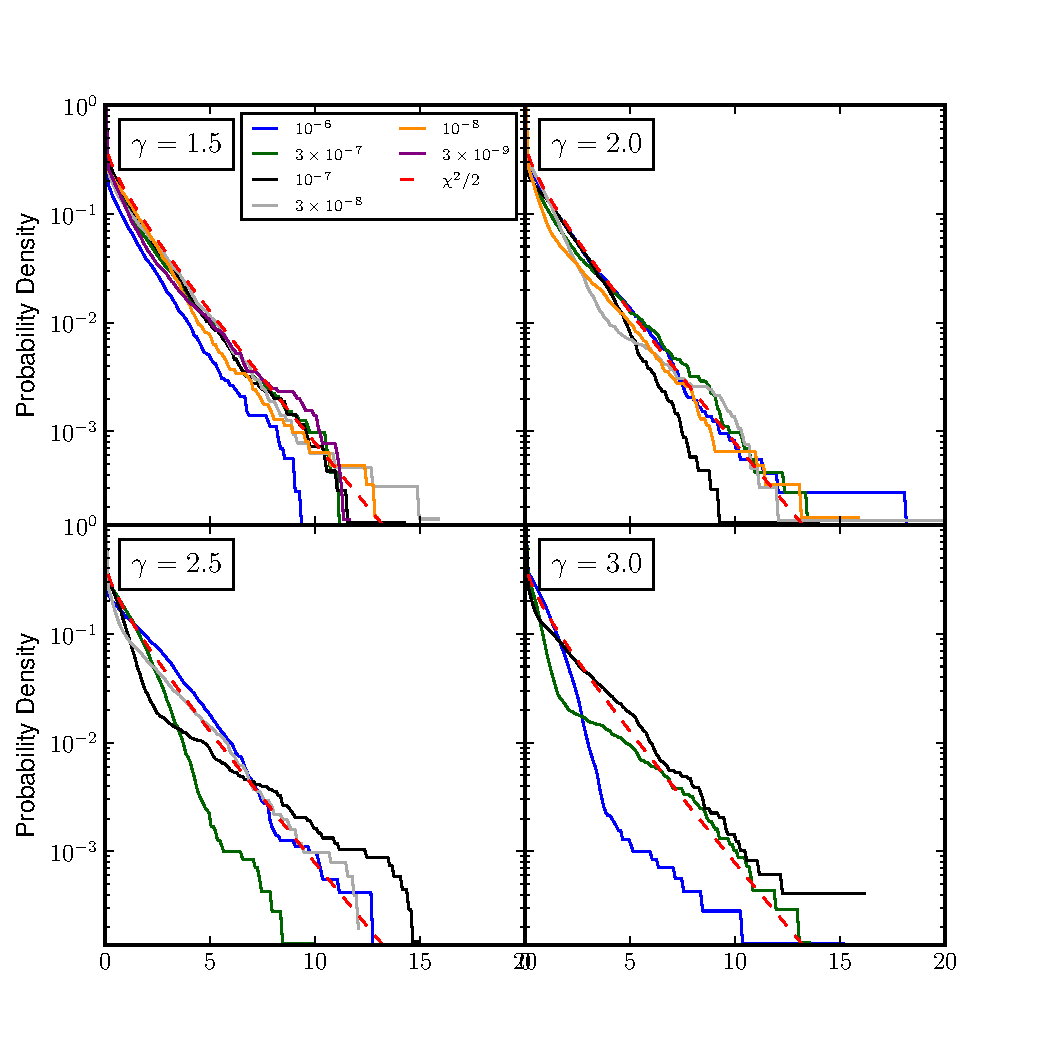
\includegraphics{mc_plots/ts_ext_emin_1000.pdf}
    % this plot came from /u/gl/lande/work/fermi/extended_catalog/monte_carlo/ts_ext/v3/plot.py
    % using data from /nfs/slac/g/ki/ki03/lande/extended_catalog/monte_carlo/ts_ext/v3_emin_1000/merged.hdf5
    \end{center}
    \caption{Lalla}\label{ts_ext}
  \end{figure}

\begin{figure}
  \begin{center}
    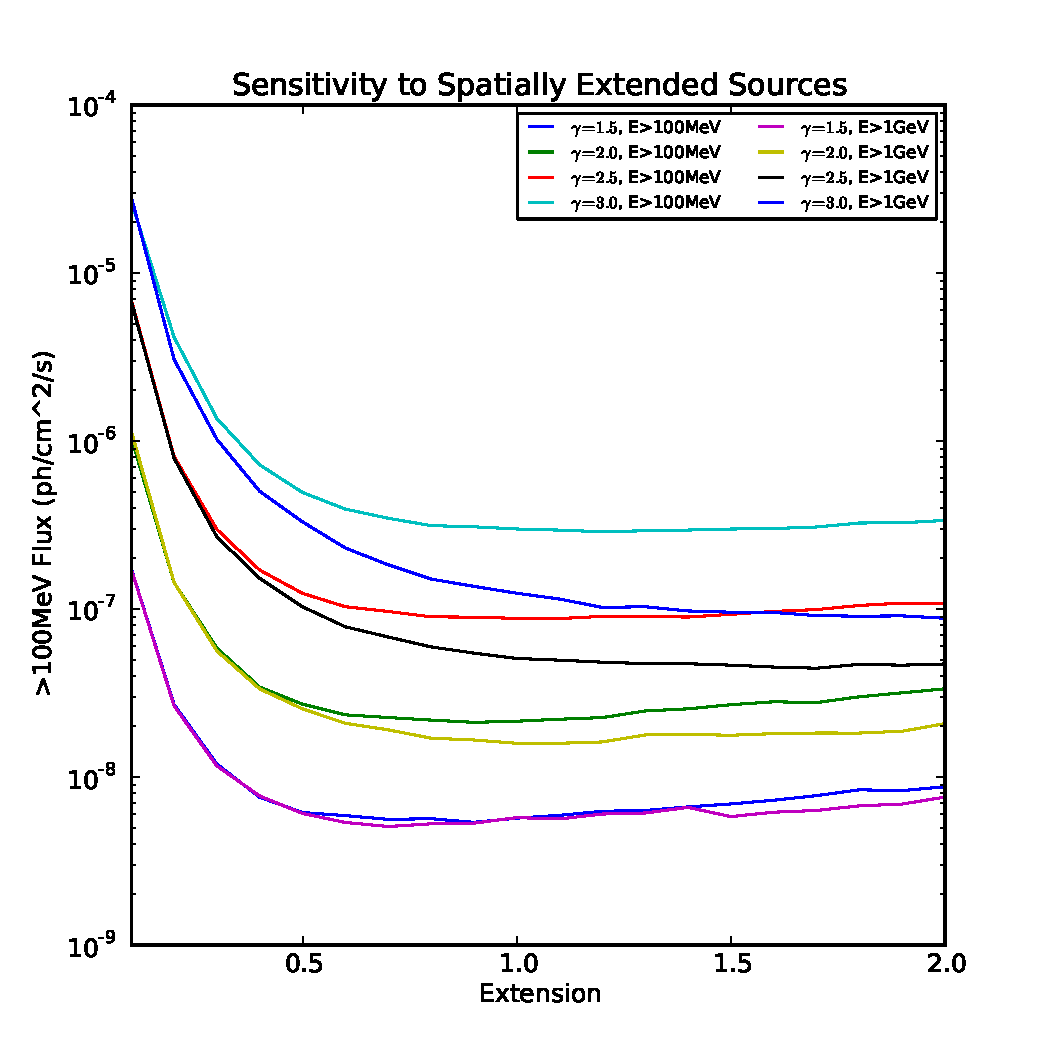
\includegraphics{mc_plots/sensitivity.pdf}
    % this plot came from /u/gl/lande/work/fermi/extended_catalog/monte_carlo/sensitivity/v8/merged_plot.py
    % using data from /nfs/slac/g/ki/ki03/lande/extended_catalog/monte_carlo/sensitivity/v7/merged.hdf5 (>1GeV)
    % using data from /nfs/slac/g/ki/ki03/lande/extended_catalog/monte_carlo/sensitivity/v8/merged.hdf5 (>100MeV)
    \end{center}
    \caption{Lalla}\label{sensitivity_ext}
  \end{figure}

  \begin{figure}
    \begin{center}
      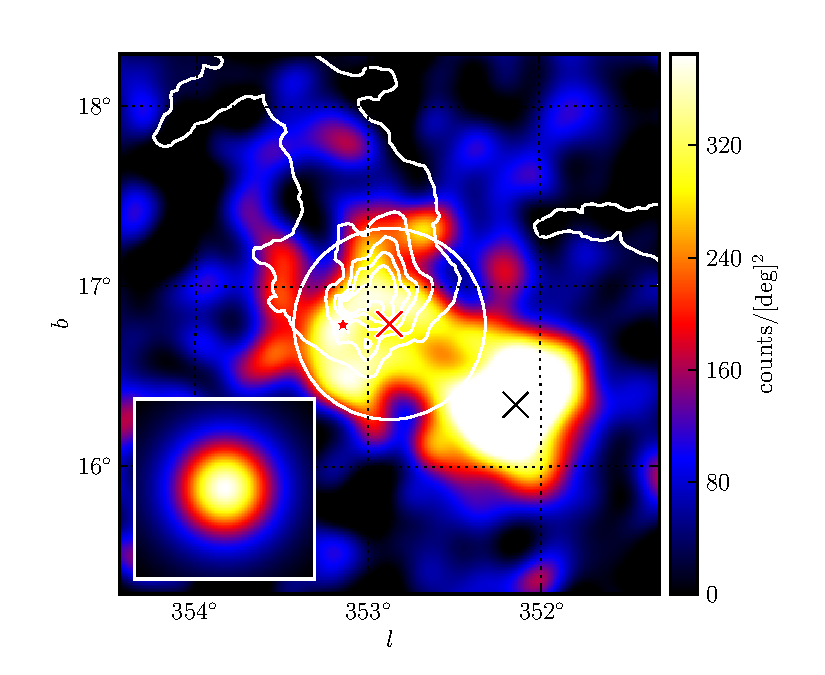
\includegraphics[type=pdf,ext=.pdf,read=.pdf]{source_plots/source_1FGL_J1628.6-2419c}
    \end{center}
    % this plot came from 
    % /nfs/slac/g/ki/ki03/lande/extended_catalog/2FGL/v10/spectral_emin_1000_v1/1FGL_J1628.6-2419c/v2/source_1FGL_J1628.6-2419c.pdf
    \caption{Lalla}
  \end{figure}

  \begin{figure}
    \begin{center}
      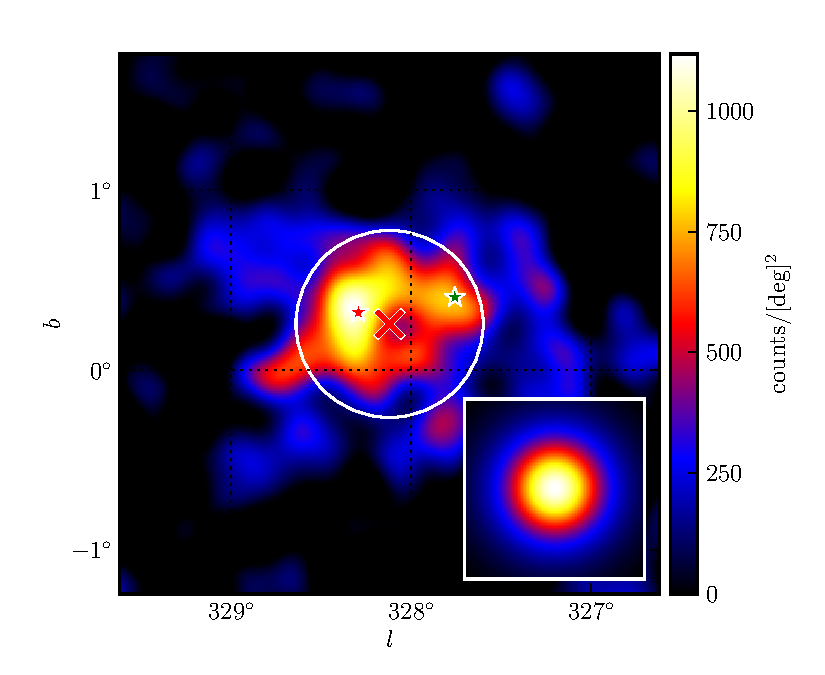
\includegraphics[type=pdf,ext=.pdf,read=.pdf]{source_plots/source_1FGL_J1554.0-5345c}
    \end{center}
    % this plot came from 
    % /nfs/slac/g/ki/ki03/lande/extended_catalog/2FGL/v10/spectral_emin_1000_v1/1FGL_J1554.0-5345c/v2/source_1FGL_J1554.0-5345c.pdf
    \caption{Lalla}
  \end{figure}

  \begin{figure}
    \begin{center}
      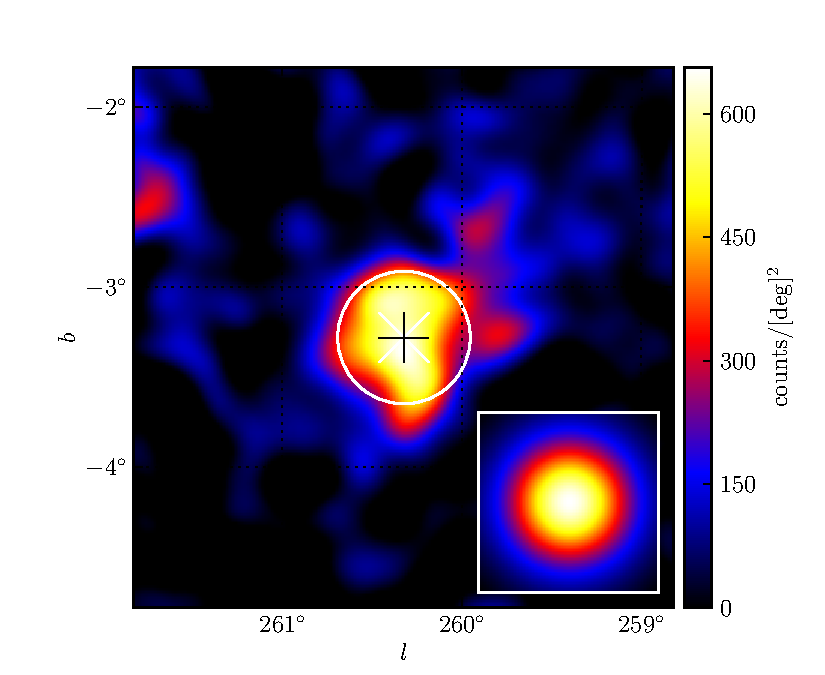
\includegraphics[type=pdf,ext=.pdf,read=.pdf]{source_plots/source_1FGL_J0823.3-4248}
    \end{center}
    % this plot came from 
    % /nfs/slac/g/ki/ki03/lande/extended_catalog/2FGL/v10/spectral_emin_1000_v1/1FGL_J0823.3-4248/v2/source_1FGL_J0823.3-4248.pdf
    \caption{Lalla}
  \end{figure}

  \begin{figure}
    \begin{center}
      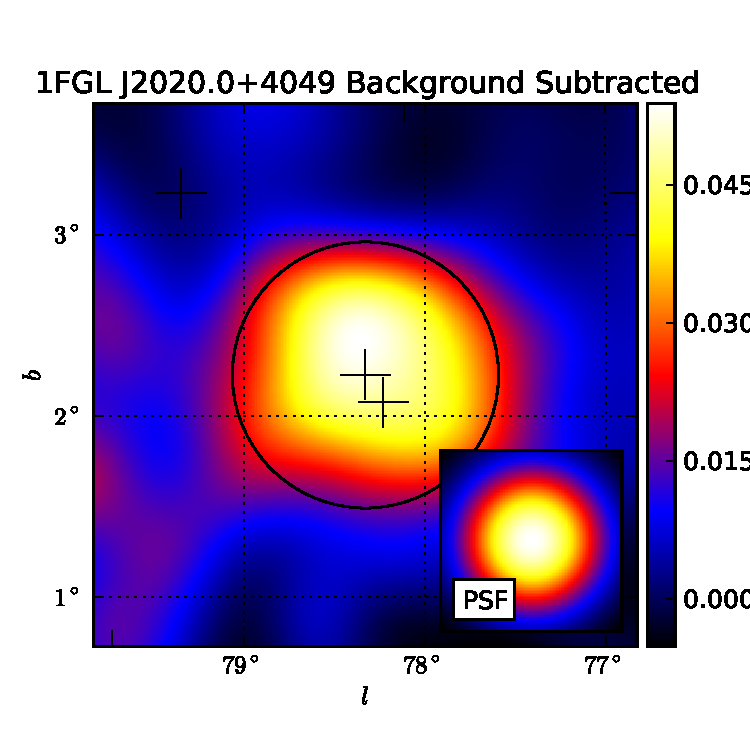
\includegraphics[type=pdf,ext=.pdf,read=.pdf]{source_plots/source_1FGL_J2020.0+4049}
    \end{center}
    % this plot came from 
    % /nfs/slac/g/ki/ki03/lande/extended_catalog/2FGL/v10/spectral_emin_10000_v1/1FGL_J2020.0+4049/v2/source_1FGL_J2020.0+4049.pdf
    \caption{Lalla}
  \end{figure}

  \begin{figure}
    \begin{center}
      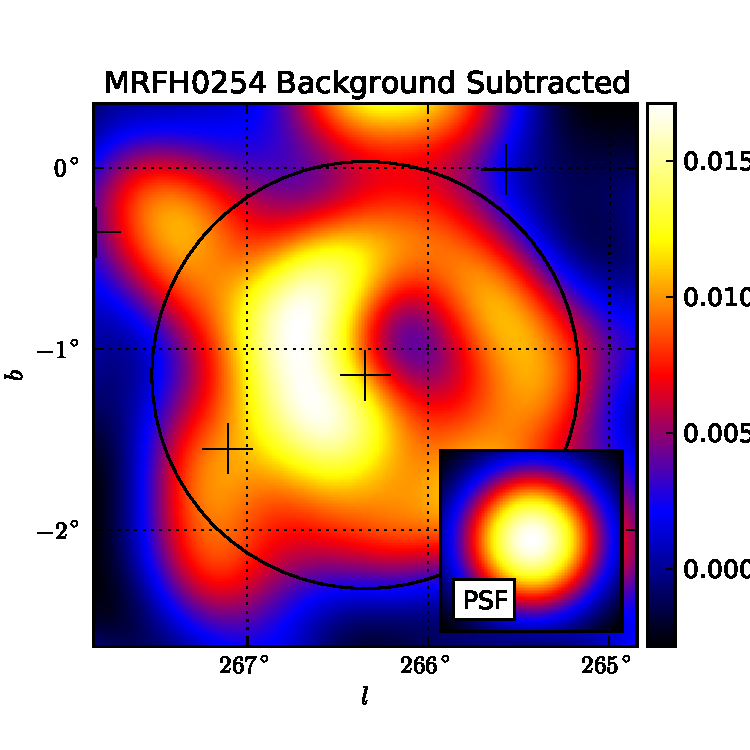
\includegraphics[type=pdf,ext=.pdf,read=.pdf]{source_plots/source_MRFH0254}
    \end{center}
    % this plot came from 
    % /nfs/slac/g/ki/ki03/lande/extended_catalog/2FGL/v10/spectral_emin_10000_v1/MRFH0254/v2/source_MRFH0254.pdf
    \caption{Lalla}
  \end{figure}

  \begin{figure}
    \begin{center}
      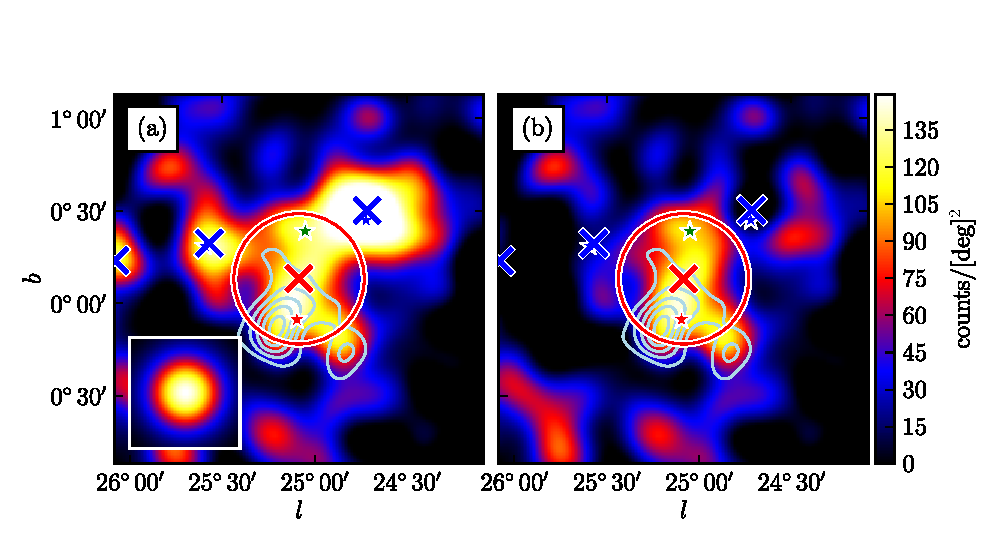
\includegraphics[type=pdf,ext=.pdf,read=.pdf]{source_plots/source_1FGL_J1837.5-0659c}
    \end{center}
    % this plot came from 
    % /nfs/slac/g/ki/ki03/lande/extended_catalog/2FGL/v10/spectral_emin_10000_v1/1FGL_J1837.5-0659c/v2/source_1FGL_J1837.5-0659c.pdf
    \caption{1FGL J1837.5-0659c}
  \end{figure}


  \begin{figure}
    \begin{center}
      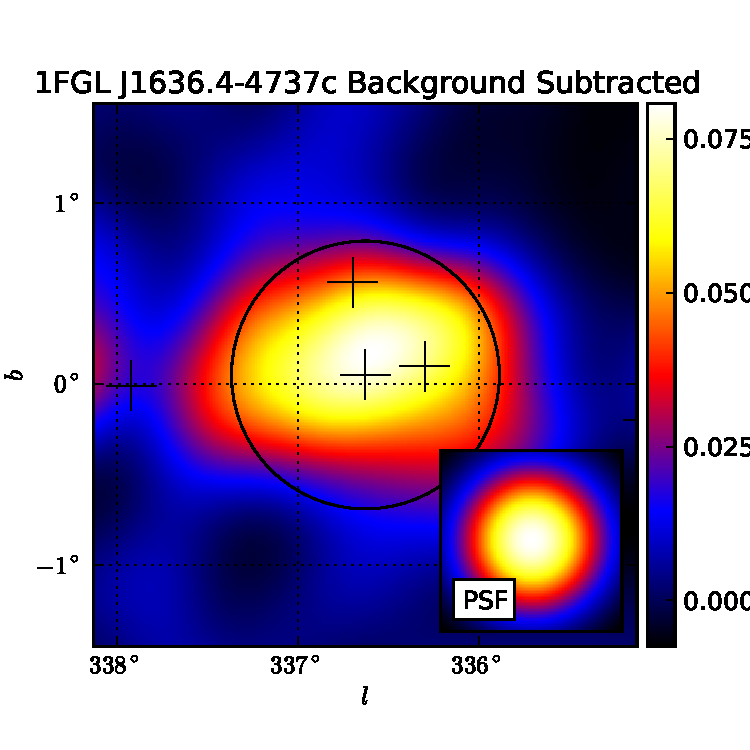
\includegraphics[type=pdf,ext=.pdf,read=.pdf]{source_plots/source_1FGL_J1636.4-4737c}
    \end{center}
    % this plot came from 
    % /nfs/slac/g/ki/ki03/lande/extended_catalog/2FGL/v10/spectral_emin_10000_v1/1FGL_J1636.4-4737c/v2/source_1FGL_J1636.4-4737c.pdf
    \caption{1FGL J1636.4-4737c}
  \end{figure}


  \begin{figure}
    \begin{center}
      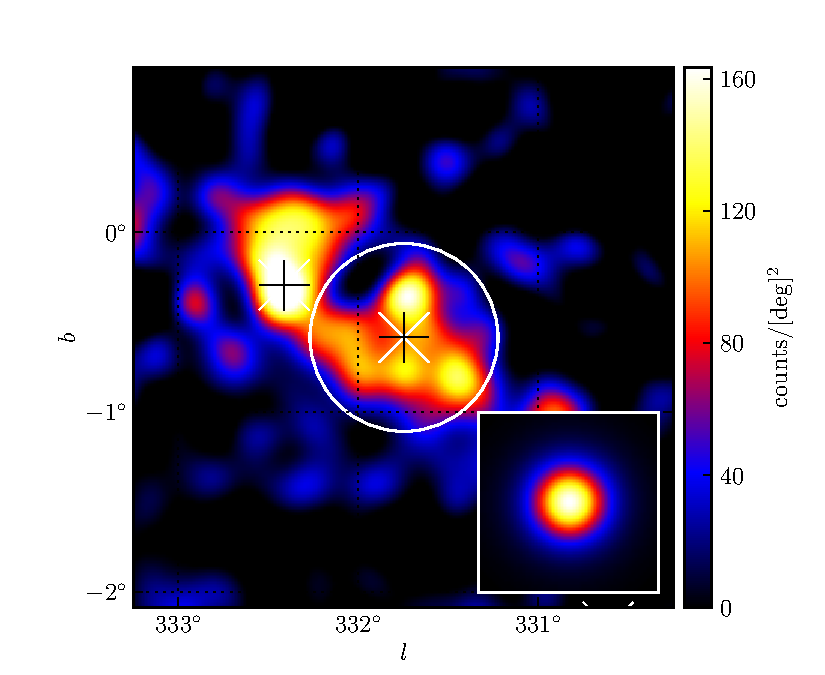
\includegraphics[type=pdf,ext=.pdf,read=.pdf]{source_plots/source_1FGL_J1613.6-5100c}
    \end{center}
    % this plot came from 
    % /nfs/slac/g/ki/ki03/lande/extended_catalog/2FGL/v10/spectral_emin_10000_v1/1FGL_J1613.6-5100c/v2/source_1FGL_J1613.6-5100c.pdf
    \caption{Lalla}
  \end{figure}




  \end{document}

